\chapter{Planification du Backlog Product}
\addcontentsline{toc}{chapter}{Planification du Backlog Product}
\markboth{Planification du Backlog Product}{Planification du Backlog Product}

\label{chap:analyseEtConception}
% section starts from 1 
%\minitoc

\section*{Introduction}
Afin de pouvoir implémentées les fonctionnalités recensées au début de ce projet, nous
s'intéressons dans ce chapitre à l'étude conceptuelle de notre application. C'est une phase de spécification et de modélisation conceptuelle basée sur le langage UML à travers les diagrammes de cas d'utilisation, les diagrammes de séquences et classes. Ceci nous permet de tracer une meilleure stratégie d'implémentation des besoins fonctionnels tout en respectant les contraintes identifiées. Ensuite, nous exposerons les besoins non fonctionnels ainsi que notre backlog de produit.

\section{Identifications des acteurs}
Un utilisateur est une entité extérieure au système de modélisation qui représente et
interagit directement avec une personne, un appareil. Chaque acteur dispose d'un ensemble
d'actions correspondant à la fonction dont il a besoin. Dans notre projet

L'application « Elise » Mobile fait intervenir plusierus acteurs comme le montre le tableau ci-après.

\begin{table}[h]
\setlength\tabcolsep{3pt}
\centering
\begin{tabularx}{\textwidth}{|c|L|}
\hline
Acteur  &  Rôles \\ 
\hline
\textbf{Collaborateur}  &  Accéde aux documents qui lui sont partagés, peut les modifier et les partager selon les tâches qui lui sont assignées \\ \hline
\textbf{Secrétaire}  &  Même rôle que le collaborateur avec en plus l'accès aux documents partagés par les autres de son service et les documents partagés par les autres services des collaborateurs \\ \hline
\textbf{Chef de service}  &  Même rôle que le secrétaire avec en plus l'accès aux documents partagés par les autres services subalternes \\ \hline
\end{tabularx}
\caption{Acteurs de l'application}
\label{tab:acteurs}
\end{table}



% note
\begin{small}
  Ces rôles/droits sont définis et appliqués par défaut par le système. Il est possible de les modifier selon les besoins spécifiques du client.
\end{small}


\section{Besoins fonctionnels des collaborateurs}
Notre application est desinée aux utilisateurs suivants : les collaborateurs, les secrétaires et les chefs de service. Chacun d'eux dispose d'un ensemble d'actions correspondant à la fonction dont il a besoin.

\begin{itemize}
% \item \textbf{Authentification} : L'utilisateur doit pouvoir s'authentifier à l'application pour pouvoir accéder à ses documents.
% \item \textbf{Consultation de profil} : L'utilisateur doit pouvoir consulter son profil.
% \item \textbf{Modification de profil} : L'utilisateur doit pouvoir modifier son profil.
% \item \textbf{Declaration d'absence} : L'utilisateur doit pouvoir déclarer son absence.
% \item \textbf{Annulation d'absence} : L'utilisateur doit pouvoir annuler son absence.
% \item \textbf{Affectation de delegé} : L'utilisateur doit pouvoir affecter un ou plusieurs délégué(s) pour le remplacer en cas d'absence.
% \item \textbf{Suppression de delegé} : L'utilisateur doit pouvoir supprimer un ou plusieurs délégué(s) affecté(s).
% \item \textbf{Recherche d'un utilisateur/service} : L'utilisateur doit pouvoir rechercher un utilisateur ou un service.
% \item \textbf{Reception de notification} : L'utilisateur doit pouvoir recevoir une notification de rappel.
% \item \textbf{Désactivation de notification} : L'utilisateur doit pouvoir désactiver les notifications.
% \item \textbf{Consulter espace de travail utilisateur} : L'utilisateur doit pouvoir consulter son espace de travail.
% \item \textbf{Consulter espace de travail personnalisé} : L'utilisateur doit pouvoir consulter son espace de travail personnalisé.
% \item \textbf{Supprimer espace de travail personnalisé} : L'utilisateur doit pouvoir supprimer son espace de travail personnalisé.
% \item \textbf{Modifier espace de travail personnalisé} : L'utilisateur doit pouvoir modifier son espace de travail personnalisé.
% \item \textbf{Ajouter un espace de travail personnalisé} : L'utilisateur doit pouvoir ajouter un espace de travail personnalisé.
% \item \textbf{Accéder aux espaces de travail de ses différents services} : L'utilisateur doit pouvoir accéder aux espaces de travail de ses différents services.
% \item \textbf{Consulter tableau de bord partagé et personnel} : L'utilisateur doit pouvoir consulter son tableau de bord partagé et personnel.
% \item \textbf{Consulter les widgets du tableau de bord personnel} : L'utilisateur doit pouvoir consulter les widgets de son tableau de bord personnel.
% \item \textbf{Ajouter un widget dans le tableau de bord personnel} : L'utilisateur doit pouvoir ajouter un widget dans son tableau de bord personnel.
% \item \textbf{Supprimer un widget dans le tableau de bord personnel} : L'utilisateur doit pouvoir supprimer un widget dans son tableau de bord personnel.
% \item \textbf{Configurer un widget du tableau de bord personnel} : L'utilisateur doit pouvoir configurer un widget de son tableau de bord personnel.
% \item \textbf{Ajouter un tableau de bord personnel} : L'utilisateur doit pouvoir ajouter un tableau de bord personnel.
% \item \textbf{Supprimer un tableau de bord personnel} : L'utilisateur doit pouvoir supprimer un tableau de bord personnel.
% \item \textbf{Modifier un tableau de bord personnel} : L'utilisateur doit pouvoir modifier un tableau de bord personnel.
% \item \textbf{Rechercher un document selon le filtre} : L'utilisateur doit pouvoir rechercher un document selon le filtre.
% \item \textbf{Accéder à l'ensemble de ses tâches} : L'utilisateur doit pouvoir accéder à l'ensemble de ses tâches.
% \item \textbf{Superviser son processus métier} : L'utilisateur doit pouvoir superviser son processus métier.
% \item \textbf{Démarrer une tâche dans un document} : L'utilisateur doit pouvoir démarrer une tâche dans un document.
% \item \textbf{Modifier informations d'un document} : L'utilisateur doit pouvoir modifier les informations d'un document.
% \item \textbf{Consulter les fichiers d'un document} : L'utilisateur doit pouvoir consulter les fichiers d'un document.
% \item \textbf{Supprimer un fichier d'un document} : L'utilisateur doit pouvoir supprimer un fichier d'un document.
% \item \textbf{Ajouter un fichier à un document} : L'utilisateur doit pouvoir ajouter un fichier à un document.
% \item \textbf{Consulter l'historique d'un document} : L'utilisateur doit pouvoir consulter l'historique d'un document.
% \item \textbf{Consulter les tâches d'un document} : L'utilisateur doit pouvoir consulter les tâches d'un document.
% \item \textbf{Supprimer une tâche d'un document} : L'utilisateur doit pouvoir supprimer une tâche d'un document.
% \item \textbf{Ajouter une tâche à un document} : L'utilisateur doit pouvoir ajouter une tâche à un document.
% \item \textbf{Consulter l'historique d'une tâche} : L'utilisateur doit pouvoir consulter l'historique d'une tâche.
% \item \textbf{Consulter les signatures} : L'utilisateur doit pouvoir consulter les signatures.
% \item \textbf{Ajouter une signature} : L'utilisateur doit pouvoir ajouter une signature.
% \item \textbf{Supprimer une signature} : L'utilisateur doit pouvoir supprimer une signature.
% \item \textbf{Signer un document manuellement} : L'utilisateur doit pouvoir signer un document manuellement.
% \item \textbf{Signer un document à l'aide des signatures enregistrées} : L'utilisateur doit pouvoir signer un document à l'aide des signatures enregistrées.

\item \textbf{Authentification}
\item \textbf{Consultation de profil}
\item \textbf{Modification de profil}
\item \textbf{Declaration d'absence}
\item \textbf{Annulation d'absence}
\item \textbf{Affectation de delegé}
\item \textbf{Suppression de delegé}
\item \textbf{Recherche d'un utilisateur/service}
\item \textbf{Reception de notification}
\item \textbf{Désactivation de notification}
\item \textbf{Consulter espace de travail utilisateur}
\item \textbf{Consulter espace de travail personnalisé}
\item \textbf{Supprimer espace de travail personnalisé}
\item \textbf{Modifier espace de travail personnalisé}
\item \textbf{Ajouter un espace de travail personnalisé}
\item \textbf{Accéder aux espaces de travail de ses différents services}
\item \textbf{Consulter tableau de bord partagé et personnel}
\item \textbf{Consulter les widgets du tableau de bord personnel}
\item \textbf{Ajouter un widget dans le tableau de bord personnel}
\item \textbf{Supprimer un widget dans le tableau de bord personnel}
\item \textbf{Configurer un widget du tableau de bord personnel}
\item \textbf{Ajouter un tableau de bord personnel}
\item \textbf{Supprimer un tableau de bord personnel}
\item \textbf{Modifier un tableau de bord personnel}
\item \textbf{Rechercher un document selon le filtre}
\item \textbf{Accéder à l'ensemble de ses tâches}
\item \textbf{Superviser son processus métier}
\item \textbf{Démarrer une tâche dans un document}
\item \textbf{Modifier informations d'un document}
\item \textbf{Consulter les fichiers d'un document}
\item \textbf{Supprimer un fichier d'un document}
\item \textbf{Ajouter un fichier à un document}
\item \textbf{Consulter l'historique d'un document}
\item \textbf{Consulter les tâches d'un document}
\item \textbf{Supprimer une tâche d'un document}
\item \textbf{Ajouter une tâche à un document}
\item \textbf{Consulter l'historique d'une tâche}
\item \textbf{Consulter les signatures}
\item \textbf{Ajouter une signature}
\item \textbf{Supprimer une signature}
\item \textbf{Signer un document manuellement}
\item \textbf{Signer un document à l'aide des signatures enregistrées}

\end{itemize}



% \section{Conception}
% \subsection{Diagramme de cas d'utilisation}
% % \begin{figure}[h]
% % \centering
% % \includegraphics[width=0.8\textwidth]{cas}
% % \caption{Diagramme de cas d'utilisation}
% % \end{figure}
% % include pdf
% Pour répondre aux besoins fonctionnels décrits ci-dessus, nous allons présenter le diagramme de cas d'utilisation global illustré dans la figure ci-dessous.
% \begin{figure}[!h]
% \centering
% 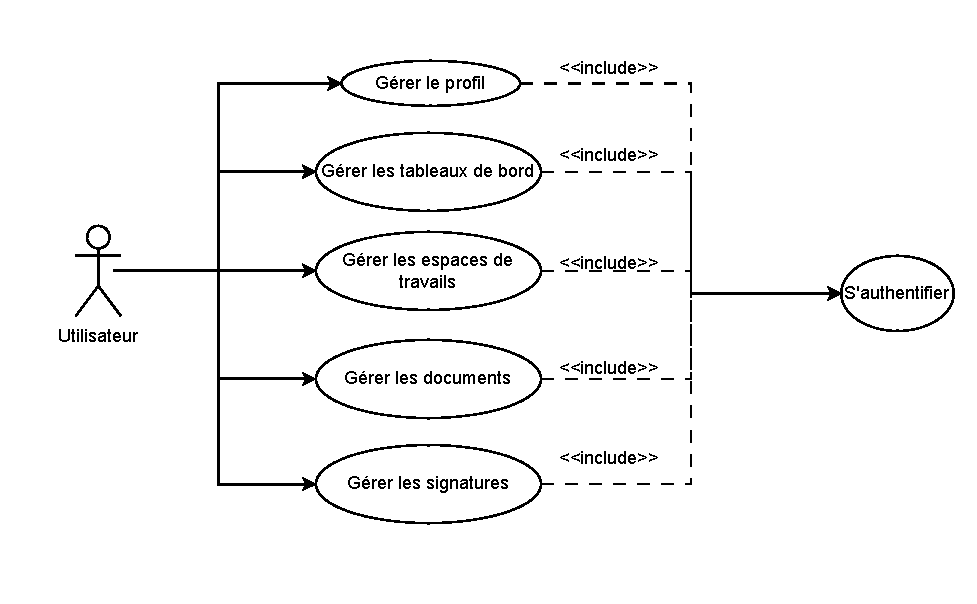
\includegraphics[width=0.6\textwidth]{useCaseGeneral}
% \caption{Diagramme de cas d'utilisation global}
% \end{figure}

% \section{Le pilotage du projet par SCRUM}
% Scrum est basé sur un ensemble de concepts permettant d'assurer une bonne gestion des projets : rôle, artefacts, sprint et réunion.

% \subsection{Identification de l'équipe SCRUM}
% L'équipe joue un rôle capital dans Scrum : elle permet d'optimiser la productivité et la
% flexibilité.

% Afin de parvenir à ces objectifs, elle doit s'auto organiser et être multi compétente. Elle doit également avoir un champ d'action suffisant pour la soutenir dans la réalisation de son travail
% Dans le contexte de notre projet, on trouve :

% \begin{itemize}
%   \item \textbf{Product Owner} Quentin DEMARTHE
%   \item \textbf{Scrum Master} Rabii MEJAI
%   \item \textbf{Equipe de développement} : Mohamed Youssef CHLENDI, Raed CHARRAD
% \end{itemize}

\section{Les User Stories}
Une user story est une expression qui décrit un point de vue de l'utilisateur et a pour objectif de donner une valeur au travail. Elle contient généralement trois éléments descriptifs de la fonctionnalité : 

  \textbf{Qui est l'utilisateur ? Qu'est-ce qu'il veut faire ? Et pourquoi veut-il le faire ?}

L'expression qui est souvent utilisée pour formuler une user story est « En tant que \textbf{'qui'}, je veux \textbf{'quoi'} afin de \textbf{'pourquoi'} ». Cette structure permet de décrire de manière concise les besoins des utilisateurs et de les prendre en compte dans la planification et le développement du produit.


% Jump page
\newpage
\begin{landscape}



  \begin{adjustwidth}{-1cm}{}
    % \usepackage{longtable}
      
      \begin{longtable}{|c|p{3cm}|p{8cm}|c|c|p{2cm}|p{2cm}|c|}
        % \centering
        \hline
    ID  &   User Story  &  Description   &  Compléxité  &  Priorité  &  Période  &  Sprint  &   \\
    % \hline
    % 1  &  Gestion d'accès et de profil  &  Texte sur une seule ligne  &  Ligne 1  &  1 \\
    \hline
    TS1  &  Formation sur la solution Elise  &  En tant que membre de l'équipe scrum, je souhaite comprendre pleinement la fonctionnalité du système Elise afin de pouvoir reproduire sa logique dans une application mobile.   &  Moyenne  &  2  &  Du 8 Février à 13  Février  &  \multirow{3}{2cm}{
      \begin{center}
        
        \textbf{Sprint 1 :} Préparation de l’environnement du travail et étude de la solution
      \end{center}
      }  &  \multirow{19}{2.5cm}[-10.5ex]{\textbf{Release 1}}  \\
    \cline{1-6}
    TS2  &  Formation en développement mobile avec Ionic Vue et Capacitor  &  En tant que scrum team, je souhaite me former au développement mobile en utilisant les technologies Ionic Vue et Capacitor. Cette formation doit me permettre de maîtriser les compétences essentielles pour créer des applications mobiles multiplateformes de qualité.  &  Moyenne  &  1  &  Du 14 Février à 21 Février  &  &  \\
    \cline{1-6}
    TS3  &  Installer et configurer l'environnement de développement  &  En tant que développeur, je veux installer et configurer le logiciel Visual Studio Code et Android studio pour travailler sur le projet en utilisant les technologies suivantes: Ionic Vue, .NET Core 6 et Capacitor.  &  Facile  &  1  &  22 Février  &  & \\

    \cline{1-7}

    TS4 & Création de signature & En tant qu'utilisateur, je veux créer une signature numérique en dessinant ma signature à l'aide de mon doigt ou de mon stylet sur l'écran tactile de mon appareil mobile, afin de pouvoir la réutiliser facilement lors de la signature de documents. & Moyenne & 2 &  & \multirow{5}{2cm}{\textbf{Sprint 2 :} 
Gestion des signatures}  &  \\

    \cline{1-6}
    TS5 & Suppression de signature & En tant qu'utilisateur, je veux supprimer une signature numérique que j'ai créée auparavant, en cas de besoin ou si ma signature a changé, afin de ne pas utiliser une signature obsolète ou inexacte. & Facile & 2 &  &  & \\

    \cline{1-6}
    TS6 & Visualisation de signature & En tant qu'utilisateur, je veux pouvoir visualiser ma signature numérique, pour m'assurer qu'elle est correcte et qu'elle convient au document en question. & Moyenne & 2 &  &  & \\

    \cline{1-6}
    TS7 & Ajout de signature à l'aide d'OCR & En tant qu'utilisateur d'Elise mobile, je veux ajouter ma signature en utilisant la reconnaissance optique de caractères (OCR), afin de gagner du temps et de faciliter le processus de signature. & Difficile & 2 &  &  & \\

    \cline{1-6}
    TS8 & Vérification d'authenticité de la signature & En tant qu'utilisateur, je veux vérifier l'authenticité d'une signature numérique ajoutée à un document, pour m'assurer que la signature est valide et qu'elle n'a pas été falsifiée ou modifiée depuis sa création. & Difficile & 2 &  &  & \\

    \cline{1-7}

    TS9&Accès aux documents&En tant qu'utilisateur, je veux accéder facilement aux documents que j'ai créés ou auxquels j'ai accès, afin de les consulter, de les modifier ou de les signer.&Moyenne&2&&\multirow{7}{2cm}{\textbf{Sprint 3 :} 
Gestion des documents}&\\

    \cline{1-6}


    TS10&Récupération des informations d'un document&En tant qu'utilisateur, je veux pouvoir récupérer les informations relatives à un document, telles que la date de création, les utilisateurs qui ont accédé au document et les tâches associées, afin de suivre l'historique du document et de mieux comprendre son contexte.&Moyenne&2&&&\\

    \cline{1-6}

    TS11&Ajout de fichiers à un document&En tant qu'utilisateur, je veux ajouter des fichiers supplémentaires à un document existant, afin de rassembler toutes les informations nécessaires dans un seul document et de faciliter le partage des informations.&Moyenne&2&&&\\
    \cline{1-6}
    TS12&Suppression d'un fichier dans un document&En tant qu'utilisateur d'Elise mobile, je veux pouvoir supprimer un fichier spécifique qui a été ajouté à un document, afin de pouvoir maintenir la pertinence et la validité des documents stockés dans l'application. &Moyenne&2&&&\\
    \cline{1-6}

    TS13&Recherche de documents&En tant qu'utilisateur, je veux rechercher des documents en utilisant différents critères, tels que le nom, la date, le type ou le contenu, afin de trouver rapidement les documents dont j'ai besoin.&Difficile&2&&&\\

    \cline{1-6}
    TS14&Afficher documents favoris&En tant qu'utilisateur, je veux affiches les favoris, afin de trouver rapidement les documents dont j'ai besoin. &Moyenne&2&&&\\

    \cline{1-6}
    TS15&Démarrage d'une tâche dans un document&En tant qu'utilisateur, je veux pouvoir démarrer une tâche dans un document en assignant une personne responsable, en définissant une date d'échéance et en ajoutant des commentaires, afin de faciliter la collaboration et le suivi des tâches.&Difficile&2&&&\\

    \cline{1-6}
    TS16&Terminaison d'une tâche dans un document&En tant qu'utilisateur, je veux pouvoir terminer une tâche dans un document en la marquant comme terminée et en ajoutant des commentaires sur le travail effectué, afin de clôturer la tâche et de faciliter le suivi du projet. &Moyenne&2&&&\\

    

    \cline{1-7}

    TS17&Visualisation de fichiers&En tant qu'utilisateur d'Elise mobile, je veux visualiser des fichiers stockés dans le document, afin de pouvoir consulter leur contenu sans avoir besoin d'une autre application ou d'un autre dispositif.&Difficile&2&&\multirow{2}{2cm}{\textbf{Sprint 4 :} Visualisation et signature de fichiers}&\\

    \cline{1-6}

    TS18&Signature de fichiers&En tant qu'utilisateur, je souhaite signer des documents électroniques de différentes manières. Je veux être en mesure de sélectionner une signature pré-enregistrée parmi celles que j'ai créées précédemment, en utilisant simplement un système de glisser-déposer pour l'appliquer au document à signer. Alternativement, je veux également pouvoir signer le document directement en utilisant une méthode de signature manuscrite, en dessinant ma signature à l'aide d'un stylet ou d'un autre périphérique d'entrée tactile.&Difficile&2&&&\\

    \cline{1-7}

    TS19&Gestion des préférences d'affichage&En tant qu'utilisateur, je veux gérer mes préférences d'affichage de l'application la couleur du thème  afin de personnaliser l'expérience utilisateur.&Moyenne&2&&\multirow{5}{2cm}{\textbf{Sprint 5 : }Gestion du Profile}&\\

    \cline{1-6}
    TS20&Gestion des préférences de notification&En tant qu'utilisateur, je veux gérer mes préférences de notification pour choisir les types de notifications que je souhaite recevoir et ceux que je ne souhaite pas recevoir afin de contrôler les informations qui me sont envoyées.&Moyenne&2&&&\\

    \cline{1-6}
    TS21&Visualisation des informations personnelles&En tant qu'utilisateur, je veux visualiser mes informations personnelles telles que mon nom, mon adresse email afin de vérifier leur exactitude et leur actualisation.&Moyenne&2&&&\\

    \cline{1-6}
    TS22&Modification des informations personnelles&En tant qu'utilisateur, je veux modifier mes informations personnelles afin de les mettre à jour en cas de changement.&Moyenne&2&&&\\

    \cline{1-6}
    TS23&Modification de la photo de profil&En tant qu'utilisateur d'Elise mobile, je veux modifier ma photo de profil pour qu'elle reflète mieux mon image professionnelle ou personnelle actuelle.&Moyenne&2&&&\\

    \cline{1-8}
    TS24&Connexion simple avec le mot de passe et l'email&En tant qu'utilisateur, je veux connecter à l'application Elise Mobile en utilisant mes identifiants (adresse e-mail et mot de passe).&Moyenne&2&&\multirow{3}{2cm}{\textbf{Sprint 6 :} Gestion d' authentifica- tion}&\multirow{11}{2.5cm}{Release 2}\\

    \cline{1-6}
    TS25&Connexion à l'aide du protocole oidc&En tant qu'utilisateur, je veux pouvoir me connecter à l'application Elise Mobile en utilisant mon compte microsoft.&Difficile&2&&&\\

    \cline{1-6}
    TS26&Déconnexion&En tant qu'utilisateur, je veux déconnecter de l'application Elise Mobile afin de protéger mes informations et données personnelles en cas de perte ou de vol de mon téléphone portable. La déconnexion doit être facile d'accès et rapide.&Moyenne&2&&&\\

    \cline{1-7}
    TS27&Déclaration d'absence&En tant qu'utilisateur, je veux déclarer une absence en spécifiant la date de début et la date de fin de mon absence, afin d'informer mes collègues et mes supérieurs hiérarchiques.&Moyenne&2&&\multirow{4}{2cm}{\textbf{Sprint 7 :}Gestion d'absence et de délégué}&\\

    \cline{1-6}
    TS28&Annulation d'une déclaration d'absence&En tant qu'utilisateur, je veux annuler ma déclaration d'absence si ma situation change et que je suis en mesure de travailler pendant la période initialement déclarée, afin de mettre à jour l'ensemble des parties prenantes informées de mon absence.&Moyenne&2&&& \\
    \cline{1-6}
    TS29&Suppression d'un délégué pendant l'absence&En tant qu'utilisateur, je veux supprimer un délégué que j'avais désigné pendant mon absence, en cas de besoin ou si je ne suis plus d'accord avec mon choix initial.&Moyenne&2&&&\\

    % \cline{1-7}
    % TS30&Ajouter des widgets de différents types&En tant qu'utilisateur, je veux pouvoir ajouter des widgets de différents types sur ma page d'accueil, afin de pouvoir suivre les informations importantes pour mon travail quotidien.&Moyenne&2&&\multirow{4}{2cm}{\textbf{Sprint 8 :}Gestion de page d'acceuil}&\\

    % \cline{1-6}
    % TS31&Supprimer les widgets existants sur ma page&En tant qu'utilisateur, je veux pouvoir supprimer les widgets existants sur ma page d'accueil, afin de pouvoir personnaliser ma page en fonction de mes besoins actuels.&Moyenne&2&&&\\

    % \cline{1-6}
    % TS32&Modifier les paramètres de chaque widget&En tant qu'utilisateur, je veux pouvoir modifier les paramètres de chaque widget, tels que le titre, la taille, la couleur et le type d'informations affichées, afin de pouvoir adapter chaque widget à mes besoins.&Difficile&2&&&\\

    % \cline{1-6}
    % TS33&Réorganiser les widgets sur ma page&En tant qu'utilisateur, je veux pouvoir réorganiser les widgets sur ma page d'accueil, afin de pouvoir mettre en évidence les informations les plus importantes en haut de la page.&Difficile&2&&&\\

    \hline
        \caption{Product Backlog}
        
      \end{longtable}
    \end{adjustwidth}
\end{landscape}

\section{Spécifications des besoins non fonctionnels}
Afin d'optimiser le fonctionnement de notre application, elle doit répondre aux différents besoins non fonctionnels présentés ci-dessous que nous devons prendre en compte afin d'assurer une meilleure utilisation et une meilleure gestion :

\begin{itemize}
\item \textbf{Performance} : L'application doit être capable de répondre aux besoins des utilisateurs en temps réel.
\item \textbf{Fiabilité} : L'application doit être fiable et ne pas présenter de dysfonctionnement, et les données fournies par l'application doivent être fiables.
\item \textbf{Usabilité} : L'application doit être facilement utilisable et compréhensible par les utilisateurs.
\item \textbf{Sécurité} : L'application doit être sécurisée et ne pas présenter de faille de sécurité.
\item \textbf{Disponibilité} : L'application doit être disponible 24h/24 et 7j/7.
\item \textbf{Maintenabilité} : L'application doit être facilement maintenable.
\item \textbf{Interopérabilité} : L'application doit être compatible avec les différents systèmes d'exploitation.
\item \textbf{Portabilité} : L'application doit être facilement portable.
\item L'application doit connecter au serveur d'application privée de l'entreprise.
\end{itemize}

% Conclusion
\section*{Conclusion}
Au cours de ce chapitre nous avons présenté les différents acteurs qui vont interagir avec notre application. Ensuite, nous avons cité les User stories, regroupées dans le Product Backlog qui décrit les fonctionnalités de chaque acteur et la répartition de ces User Stories en sprints et en différents releases. Et enfin nous avons défini les besoins non fonctionnels de notre solution.